\chapter{Variants of the Basic Convolution Function}

In the context of neural networks, we do not usually apply the standard convolution operation, as presented in Chapter \labelcref{ch:what-is-conv}. The convolution operation at the core of CNNs admits several useful modifications that expand its flexibility and efficiency.  
The variants of the basic convolution functions can differ slightly in how parameters are shared, how receptive fields are enlarged or how the computation is factorized.  

\section{Strided convolution}

When dealing with images, software implementations usually work in batch mode, so they use as input and output of the convolution some 4-D tensors, with the first index into the different channels, the following two indices into the spatial coordinates of each channel and the fourth axis indexing different examples in the batch. 

Assume we have 4-D kernel tensor $K$ with element $K_{i,j,k,l}$ giving the connection strenght between a unit channel in channel $i$ of the output and a unit in channel $j$ of the input, with an offset of $k$ rows and $l$ columns between the output unit and the input unit. Assume our input consists of observed data $v$ with element $V_{i,j,k}$ giving the value of the input within channel $i$ at row $j$ and column $k$. Assume our output consists of $Z$ with the same format as $V$. If $Z$ is produced by convolving $K$ across $V$ without flipping $K$, then:

\begin{equation}
    Z_{i,j,k}=\sum_{l,m,n}V_{l,j+m-1,k+n-1}K_{i,l,m,n}
\end{equation}

where the summation over $l, m$ and $n$ is over all values for which the tensor indexing operations inside the summation are valid.

In standard convolution, the kernel is applied at every possible location in the input. A simple modification consists of applying the kernel only at locations separated by a fixed step size, known as the \textit{stride}. Formally, for stride $s$, the output of the convolution is defined only at positions spaced $s$ units apart:

\begin{equation}
    Z_{i,j,k}=c(K,V,s)_{i,j,k}=\sum_{l,m,n}[V_{l,(j-1)\times s+m,(k-1)\times s+n}K_{i,l,m,n}]
\end{equation}
 
\clearpage

This reduces the spatial resolution of the output and combines the effects of convolution and subsampling. We already saw that \textit{strided convolution} is often used as an alternative to pooling, section \labelcref{sec:pooling-alternatives}.  

\section{Zero-padding}

Another common variant is related to the ability of \textit{zero-padding}, where the input is padded with zeros around its border before applying convolution, to make it wider. Zero-padding allows control over the size of the output feature maps.  
Without padding, the spatial dimensions shrink after each convolution; with appropriate padding, the output can be kept at the same size as the input.

\begin{figure} [H]
    \centering
    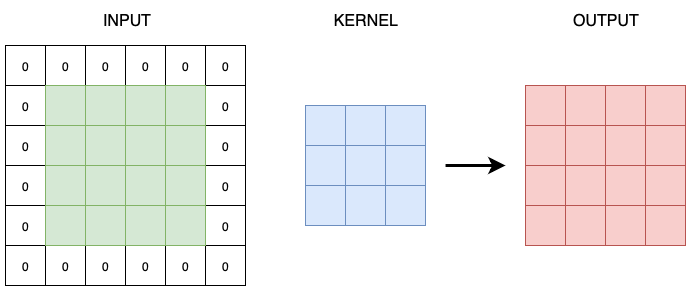
\includegraphics[width=0.7\linewidth]{Images//Chapters/zero_padding.png}
    \caption{Example of zero padding equal to one.}
    \label{fig:zero_padding}
\end{figure}

The most common conventions are: \textbf{valid convolution} in which no padding is applied, so for a one-dimensional input of length $m$ convolved with a kernel of size $k$ the output length is $m - k + 1$; \textbf{same convolution} where padding is chosen so that the output has the same size as the input, i.e.\ $m$; \textbf{full convolution}, here padding is added so that the kernel can be applied at every possible shift, producing an output of size $m + k - 1$.  

\section{Unshared and Tiled Convolution}

In a standard convolutional layer, the same kernel is applied across all spatial locations. This weight sharing greatly reduces the number of parameters.  
However, we can relax this assumption, leading to the concept of \textit{locally connected layers}.  

The most general case is the \textbf{unshared convolution} where each output unit has its own distinct set of weights rather than sharing the same kernel across all positions.

\clearpage

Formally, let $x \in \mathbb{R}^{n}$ be a one-dimensional input and suppose we use windows of size $k$ to produce an output $y \in \mathbb{R}^{m}$.  
In a standard convolution, the same kernel $w \in \mathbb{R}^{k}$ is used at all locations. In the unshared case, each position $i$ has its own kernel $w^{(i)} \in \mathbb{R}^{k}$, yielding:

\begin{equation}
y_i = \sum_{j=1}^{k} w^{(i)}_j \, x_{i+j-1}, \quad i=1,\dots,m.
\end{equation}

This increases the number of parameters from $k$ to $m \times k$, and in higher dimensions from $k^2$ to $m \times n \times k^2$, making the model far less efficient.  
Locally connected layers are useful when we know that each feature should be a function of a small part of space, but there is no reason to think that the same feature should occur across all of space. 

Between the two extremes of full parameter sharing (\textit{standard convolution}) and no sharing (\textit{unshared convolution}), there exists an intermediate approach known as \textbf{tiled convolution}.  
In this variant, weights are shared, but only among a restricted set of positions.  
For example, one might specify a tiling factor $t$, such that every $t$ consecutive locations reuse the same kernel, after which a new set of weights is introduced.  

Formally, let $w^{(1)}, \dots, w^{(t)}$ denote $t$ different kernels.  
At position $i$, the kernel used is determined by $w^{(i \bmod t)}$, i.e.

\begin{equation}
y_i = \sum_{j=1}^{k} w^{(i \bmod T)}_j \, x_{i+j-1}.
\end{equation}

This design relaxes the strong prior of full translation equivariance while still controlling the number of parameters compared to the fully unshared case.  
It allows the model to learn features that vary smoothly across space, without requiring each location to have an entirely independent set of weights.  

Locally connected and tiled convolutional layers exhibit a particular interaction with max pooling: their detector units rely on distinct filters. When these filters capture different transformed versions of the same feature, the subsequent max pooling operation produces units that are invariant to such transformations. (Figure \labelcref{fig:pooling_invariance}).  

\section{Separable convolution}

A kernel can sometimes be factorized into simpler components.  
For example, a 2D convolution with a $k \times k$ kernel can be replaced by two 1D convolutions ($k \times 1$ followed by $1 \times k$).  
This is known as \textbf{spatially separable convolution} and it reduces computation when the factorization is exact or a good approximation.  

\clearpage

An important extension is the \textit{depthwise separable convolution}, introduced in MobileNets, 2017 \cite{howard2017mobilenets}.  
This factorizes convolution into two steps:  
\begin{enumerate}
    \item a \textit{depthwise convolution}, where each filter is applied independently to a single input channel;  
    \item a \textit{pointwise convolution}, using $1 \times 1$ kernels to combine information across channels.  
\end{enumerate}
This decomposition greatly reduces the number of parameters and multiplications, enabling efficient CNNs suitable for mobile and embedded devices.